\section{Image Acquisition}

% input domains
Since one premise of the system is that hand-drawn sketches are compared with a
large body of images from various sources, a division into two input domains
seems obvious. The first domain, the domain of query sketches, is quite narrow,
because we can characterize its members as binary images with large, smooth
areas separated by discontinuities along curves. The database images, that make
up the second domain, are not subject to such limitations. They may be color
photographs (\autoref{fig:input_example_color}), paintings, computer renderings
or black-and-white sketches.

\paragraph{LUMA}

Because the Fast Discrete Curvelet Transform used in every variant of the
signature extraction step takes a single 2D matrix as input, images with more
than one color channel need to be reduced to one channel. The RGB values from
the benchmark dataset have therefore been converted to greyscale images using
the definition of luma according to ITU standards \autocite{_parameter_2002}
(\autoref{fig:input_example_luma}).  Each pixel with red, green and blue values
$(R, G, B)$ is mapped to a luminance value $Y$ using
\begin{equation*}
    Y = \frac{299}{1000}R + \frac{587}{1000}G + \frac{114}{1000}B.
\end{equation*}

\paragraph{SOBEL}

In order to make comparing the query sketch to the database images more
effective, an edge extraction algorithm can be applied to each database image.
The Sobel operator calculates horizontal and vertical gradients by convolving
the image with the $3 \times 3$ kernels
\begin{equation*}
    K_x =
    \begin{bmatrix}
        -1 & 0 & 1 \\
        -2 & 0 & 2 \\
        -1 & 0 & 1
    \end{bmatrix}
    \text{ and }
    K_y =
    \begin{bmatrix}
        -1 & -2 & -1 \\
         0 &  0 &  0 \\
         1 &  2 &  1
    \end{bmatrix}
\end{equation*}
to obtain the directional gradients $G_x$ and $G_y$. The overall response is
the gradient magnitude $G$ at each pixel location
(\autoref{fig:input_example_sobel}):
\begin{equation*}
    G = \sqrt{G_x^2 + G_y^2}
\end{equation*}

\paragraph{CANNY}

A slightly more complex way to extract edges is the Canny edge detector
\autocite{canny_computational_1986}. Initially, the image is smoothed via a
convolution with a small Gaussian kernel to reduce the susceptibility to noise,
even though this increases the localization error of the edge detection. On the
smoothed image the gradient magnitude is calculated using the Sobel operator
described above. The angle of the gradient can be calculated from the
directional gradients $G_x$ and $G_y$ using
\begin{equation*}
    \Theta = \arctan{\frac{G_x}{G_y}}
\end{equation*}
and quantized into bins for $0 \degree$, $45 \degree$, $90 \degree$ and $135
\degree$. Thin edges can be obtained from the gradient magnitudes by performing
non-maximum suppression along the direction perpendicular to the gradient
direction, e.g. a pixel is marked as being on a $90 \degree$ edge if its
magnitude is larger than the magnitudes north and south of its location. To
avoid lines being broken up by noisy fluctuations, the edges are traced along
their direction and gaps are filled in if the signal within the gap is above a
certain threshold. The result is a binary edge map of the whole image
(\autoref{fig:input_example_canny}).

\paragraph{SEGMENT}

What a human sketches as a line in an image is often a boundary between two
regions with different color or texture characteristics. Therefore the output
from image segmentation algorithms can also indicate the location of edges. The
hierarchical segmentation algorithm gPb-owt-ucm published by Arbeláez et al.\ 
\autocite{arbelaez_contours_2009} \autocite{arbelaez_contour_2011} was chosen
because it represents the most recent advances in contour detection and it
incorporates both local and global image information. On the gPb contour
detector described in \autoref{sec:background_gpb} they apply the Oriented
Watershed Transform, that merges adjacent regions of an over-segmented image.
The criterion for merging is the strength of the boundary shared by the two
regions.

\begin{figure}[h]
    \centering
    \subfloat[Original image]{%
        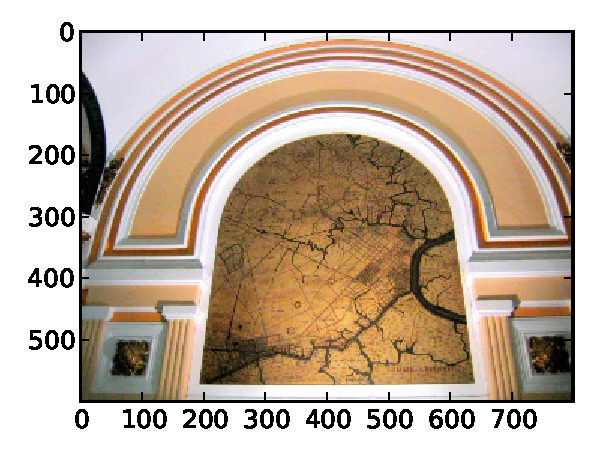
\includegraphics[width=0.55\textwidth]{input_example_color}%
        \label{fig:input_example_color}%
    }
    \quad
    \subfloat[Image after luma conversion]{%
        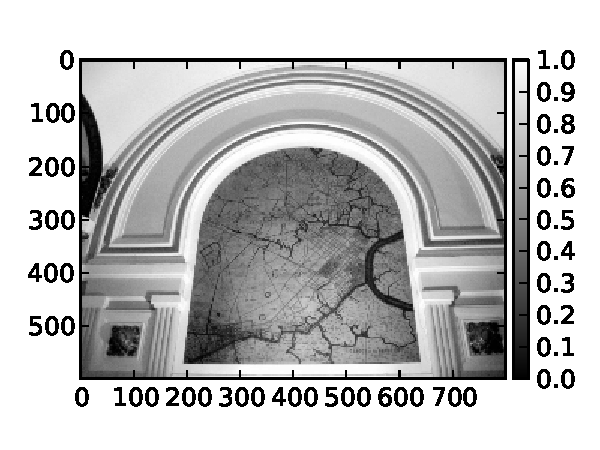
\includegraphics[width=0.45\textwidth]{input_example_luma}%
        \label{fig:input_example_luma}%
    }
    \quad
    \subfloat[Image after Sobel operator]{%
        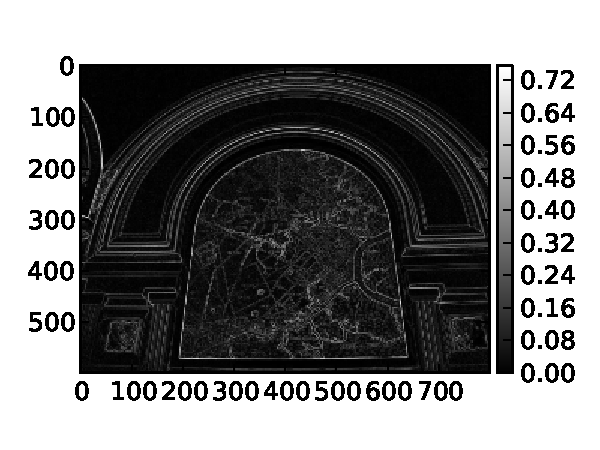
\includegraphics[width=0.45\textwidth]{input_example_sobel}%
        \label{fig:input_example_sobel}%
    }
    \quad
    \subfloat[Image after Canny operator]{%
        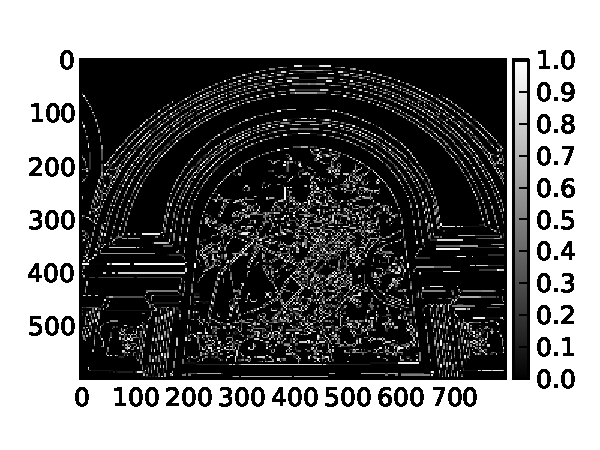
\includegraphics[width=0.45\textwidth]{input_example_canny}%
        \label{fig:input_example_canny}%
    }
    \quad
    \subfloat[Image after gPb contour detection]{%
        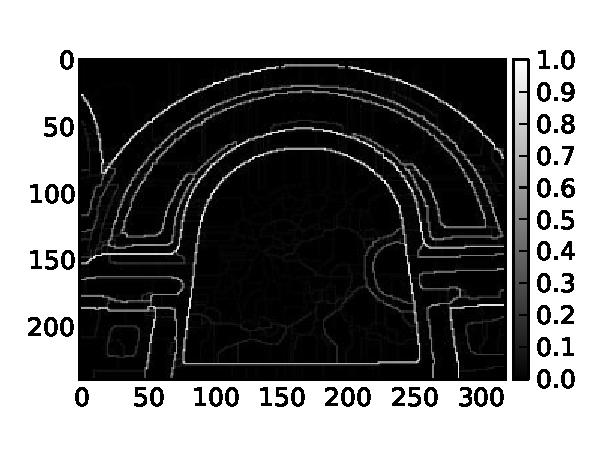
\includegraphics[width=0.45\textwidth]{input_example_segment}%
        \label{fig:input_example_segment}%
    }
    \caption[Image acquisition variants]{
        Image acquisition variants
    }
    \label{fig:input_examples}
\end{figure}
